\documentclass{article}
\usepackage{times}
\usepackage{graphicx}
\usepackage{subfigure} 
\usepackage{natbib}
\usepackage{algorithm}
\usepackage{algorithmic}
\usepackage{subfigure}
\usepackage{hyperref}
\newcommand{\theHalgorithm}{\arabic{algorithm}} % Fixes misbehavior of conflicting packages.
\usepackage{icml2016/icml2016} 
\usepackage[nolist]{acronym} % Acronym package -- give argument <dua> to suppress acronym usage


\icmltitlerunning{Approximate State Abstraction}

% --- Notation Commands ---
\newcommand{\ep}{\widetilde \phi}

% --- Note Commands ---
\usepackage{color}
\newcommand\dnote[1]{\textcolor{blue}{Dave: #1}}
\newcommand\enote[1]{\textcolor{green}{Ellis: #1}}

% --- DOCUMENT ---
\begin{document}

\twocolumn[
\icmltitle{Approximate State Abstraction}

% Paper Meta Info
\icmlauthor{David Abel}{david_abel@brown.edu}
\icmladdress{Brown University,
            115 Waterman Street, Providence, RI 02906}
\icmlauthor{D. Ellis Hershkowitz}{david_hershkowitz@brown.edu}
\icmladdress{Brown University,
            115 Waterman Street, Providence, RI 02906}
\icmlauthor{Michael L.\ Littman}{michael_littman@brown.edu}
\icmladdress{Brown University,
            115 Waterman Street, Providence, RI 02906}
    
\icmlkeywords{Reinforcement Learning, State Aggregation, State Abstraction, Planning, MDP}
            
\vskip 0.3in
]


%Acronyms -- use \ac for acronym or \acp for plural/capitalization of acronym
\begin{acronym}
\acro{MDP}{Markov Decision Process}
\acrodefplural{MDP}[MDPs]{Markov Decision Processes}

\acro{RL}{reinforcement learning}
\acrodefplural{RL}{RL}{Reinforcement learning}
\end{acronym}


% --- ABSTRACT ---
\begin{abstract}
The combinatorial explosion that plagues planning and \ac{RL} algorithms can be reversed using abstraction. For instance, prohibitively difficult task representations can be condensed so that solutions are tractably computable. In this work, we investigate a theoretical framework for approximate state abstraction that preserves near optimal behavior. \acp{RL} agents using these abstractions may treat experiences that resemble each other as equivalent, and generalize knowledge to novel scenarios based on prior experiences. We present theoretical guarantees of the quality of value functions derived from four classes of approximate state abstraction. Additionally, we empirically evaluate the relationship between the degree of approximation and the degree of abstraction achieved, as well as the tradeoff between approximation magnitude and optimality of behavior.
\end{abstract}

% Set of actions within epsilon (Q*) is the same for two states? Better than boltzmann.


% --- SECTION: Introduction ---
\section{Introduction}
Abstraction is a fundamental tool of intelligent agent seeking to compute over only the salient features of its environment. However, the knowledge available to an agent at any given moment is typically approximate and so agents are faced with the challenge of deciding when their knowledge is sufficiently accurate to form the basis of abstraction. This work focuses on characterizing what ``sufficiently accurate" information for abstraction amounts to in the context of planning and \ac{RL} in \acp{MDP}.

Solving for optimal behavior in \acp{MDP} in a planning setting is known to be P-Complete in the size of the state space CITE MICHAEL COMPLEXITY PAPER. Similarly, many \ac{RL} algorithms for solving MDPs are known to require a number of samples polynomial in the size of the state space CITE SOME SAMPLE COMPLEXITY PAPER. Although polynomial runtime or sample complexity is often what one hopes, due to Bellman's so-called curse of dimensionality the state space of an MDP often grows super-polynomially with the number of variables that characterize the domain. Thus, polynomial behavior in state space size is not necessarily the \enote{bee's knees}. For instance, a robot involved in a pick and place task might be able employ planning algorithms to solve for how to manipulate some objects into a desired configuration in time polynomial in the number of states, but the number of states it must consider to do so grows exponentially with the number of objects it plans over CITE DABE ICAPS.

Thus, a key research interest of planning and RL has been leveraging abstraction as means of grappling with large state spaces (CITE VARIOUS ABSTRACTION JOANT). These methods are characterized by reducing \textit{ground} MDPs with large state spaces to \textit{abstract} MDPs with smaller state spaces by aggregating states with similar values of interest. Existing work has characterized how aggregation of states with equal values of particular quantities fully maintain optimality CITE LIHONG. However, exactly solving for these quantities is itself computationally taxing and sometimes as difficult as solving for optimal behavior in the ground MDP, thereby defeating the purpose of abstraction.

In this work we demonstrate that aggregation of states on the basis of various approximately equal criteria incur bounded error.  Relaxing the aggregation criteria from equality of quantities to epsilon-closeness offers two benefits. First, state aggregation algorithms that satisfy these criteria employ the sort of knowledge which we might reasonably a planning or learning algorithm to approximate without fully solving the MDP. Second, because the state aggregation criteria are relaxed to approximate equality, methods which employ approximate equality are able to tune the aggressiveness of state aggregation all the while incuring bounded error.
	
\enote{QUICK SUMMARY OF PAPER PARAGRAPH}

%\begin{itemize}
%\item Solving MDPs is P-Complete, where the dominant factor is $|\mathcal{S}|$.
%\item Sample complexity is {\it also} dominated by $|\mathcal{S}|$.
%\item To make MDPs with large $|\mathcal{S}|$ tractable, we can reduce the MDPs to a simpler form.
%\item In this work, we show that compressing MDPs in a particular way allows for the transfer of bounded-error solutions between the compressed MDP and ground MDP.
%\item Q: Why approximate?
%\item A: Approximate can compress strictly more than compression based on equality
%\item A: Approximate compression requires the type of knowledge that we could imagine learning (i.e.. approximate knowledge)
%\end{itemize}

% --- SECTION: Background ---
\section{Background}

%MDP/SDM Background and Notation
\subsection{\acp{MDP} and Sequential Decision Making}
A \ac{MDP} is a five-tuple: $\langle \mathcal{S}, \mathcal{A}, \mathcal{T}, \mathcal{R}, \gamma \rangle$: $\mathcal{S}$ is a finite state space; $\mathcal{A}$ is the set of actions available to the agent; $\mathcal{T}$ denotes $\mathcal{T}(s' \mid s,a)$, the probability of an agent applying action $a \in \mathcal{A}$ in state $s \in \mathcal{S}$ and arriving in $s' \in \mathcal{S}$; $\mathcal{R}(s)$ denotes the reward received by the agent arriving in state $s$; $\gamma \in [0, 1]$ is a discount  factor that defines how much the agent prefers immediate rewards over future rewards.

The goal of an agent in an \ac{MDP} is to solve for a policy that maps states to actions: $\pi: \mathcal{S} \rightarrow \mathcal{A}$. In particular, the agent wants to solve for the policy that maximizes its expected discounted reward from any state. This goal policy is denoted $\pi^*$. We denote the expected discounted reward for following policy $\pi$ from state $s$ as the value of the state under that policy, $V(s)^\pi$. We similarly denote the expected discounted reward for taking action $a \in \mathcal{A}$ and then following policy $\pi$ from state $s$ forever after as $Q^\pi(s,a)$. Lastly, we denote the value and $Q$ functions under the optimal policy as $V^*$ and $Q^*$ respectively.

%Lihong Section
\subsection{Abstraction Notation}
We build upon the notation used by \cite{li2006towards} \enote{This should probably say more}.
We understand an abstraction as a mapping from a ground MDP $M_G$ to an abstract MDP $M_A$ using a state aggregation scheme. $M_G = \langle \mathcal{S}_G, \mathcal{A}, \mathcal{T}_G, \mathcal{R}_G, \gamma \rangle$ and $M_A = \langle \mathcal{S}_A, \mathcal{A}, \mathcal{T}_A, \mathcal{R}_A, \gamma \rangle$. 

The states in the abstract MDP are constructed by applying a state aggregation scheme, $\phi$, to the states in the ground MDP. $\mathcal{S}_A$


% Quick MDP blurb?

% Phi notation

% Evluation of Abstract MDP

% Abstract MDP, Ground MDP, Homogenizing Gun

% Previous state aggregation stuff? Or should be in related work?


% --- SECTION: Related Work ---
\section{Related Work}

% Lihong/Walsh/Littman: Towards a unified theory...
Citation test~\cite{li2006towards}

\begin{itemize}
\item ALisp~\cite{andre2002state}

Programming language for enabling abstraction.

\item Aggregation in DP~\cite{Bean2011}

Assumes the MDP is a DAG. Only does shortest path.

\item New Operators for RL~\cite{Bellemare2015}

Comes up with an approximate Bellman Operator. Not sure how it's related yet.

\item DP with Factored Representations~\cite{Boutilier2000}

Uses decision trees and DBNs to represent MDPs. Does state aggregation. Theorem 4.4 should be looked at in more detail.

\item {\bf Model reduction techniques for nearly optimal MDP solutions}~\cite{dean1997model}

$\epsilon$-homogeneity: groups together states that behave approximately the same under all or some subset of policies.

Bounded Parameter MDP: family of MDP with upper and lower bounds on T. Find policies approximately optimal w.r.t. original MDP.
% Also covers model minimization..

\item Abstraction selection~\cite{jiang2015abstraction}

\item State abstraction discovery from irrelevant state variables~\cite{jong2005state}

\item Selecting the state rep in RL~\cite{maillard2011selecting}

\item Near optimal state reps~\cite{ortner2014selecting}

\item SMDP homomorphisms~\cite{ravindran2003smdp}

\end{itemize}

% Nan/Lihong

% Approximate bisimulation

% David Silver: Options/State Abstraction?

% Russell? PHAM/HAM/ALisp

% Konidaris? Options induce symbolic representation on continuous state space

% Littman: Relocatable Action Models

% Stone: State Abstraction Discovery from Irrelevant State Vars

% Others...




% --- SECTION: State Abstraction ---
\section{Approximate State Abstraction}

% Explain each of the Phis

% One theorem, each separate phi is its own lemma.


% Subsections for proofs for each phi
\dnote{Insert lemma for each phi as their subsection}

% Subsection: 

% Subsection: Phi_Q
\subsection{$\phi_{Q^*}$}

% Subsection: Phi_M
\subsection{$\phi_{model}$}

% Subsection: Phi_{Mult}
\subsection{$\phi_{mult}$}

% Subsection: Phi_B
\subsection{$\phi_{bolt}$}

% Subsection: Other Abstractions
\subsection{Other Abstractions}

% Discussion of other abstractions we looked into

% Some abstractions DON'T preserve a meaningful notion of optimality.



% --- SECTION: Example Domains ---
\section{Example Domains}

\dnote{For each section, we'll include a plot comparing $\epsilon$ to \# states, and $\epsilon$ to performance. For UpWorld and NChain, we can include visuals of uncompressed and compressed (not useful for trench).}

% Subsection: UpWorld
\subsection{UpWorld}

\dnote{As part of UpWorld we can include the result about the unbounded improvement in sample complexity (small lemma or something?)}

% Insert visual and/or stats on number of states and performance of VI solving the abstract MDP and evaluating the resulting policy on the original MDP


% Subsection: NChain
\subsection{NChain}

% Insert visual and/or stats on number of states and performance of VI solving the abstract MDP and evaluating the resulting policy on the original MDP


% Subsection: Trench
\subsection{Trench}

% Insert visual and/or stats on number of states and performance of VI solving the abstract MDP and evaluating the resulting policy on the original MDP


% Figure: The Trench Problem
\begin{figure}[h]
\centering
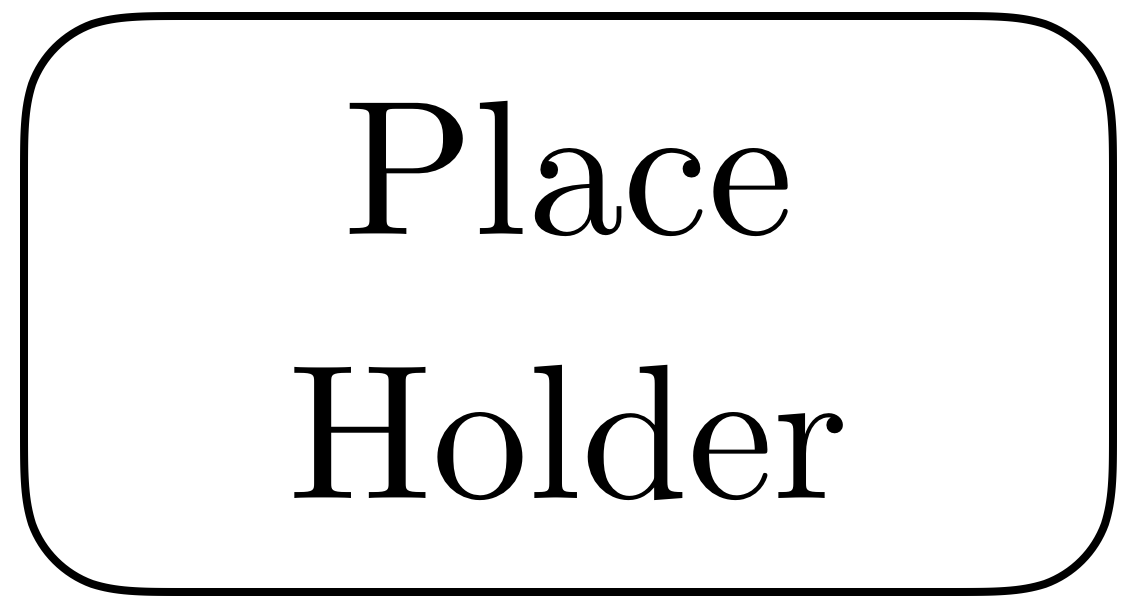
\includegraphics[width=0.42\columnwidth]{figures/placeholder.png}
\caption{The Trench Problem}
\label{fig:trench}
\end{figure}


% --- SECTION: Approximate Abstraction on Example Domains ---
\section{Approximate Abstraction on Example Domains}

% Figure: Epsilon vs. #States for all three sample domains.
\begin{figure}
\subfigure[UpWorld]{
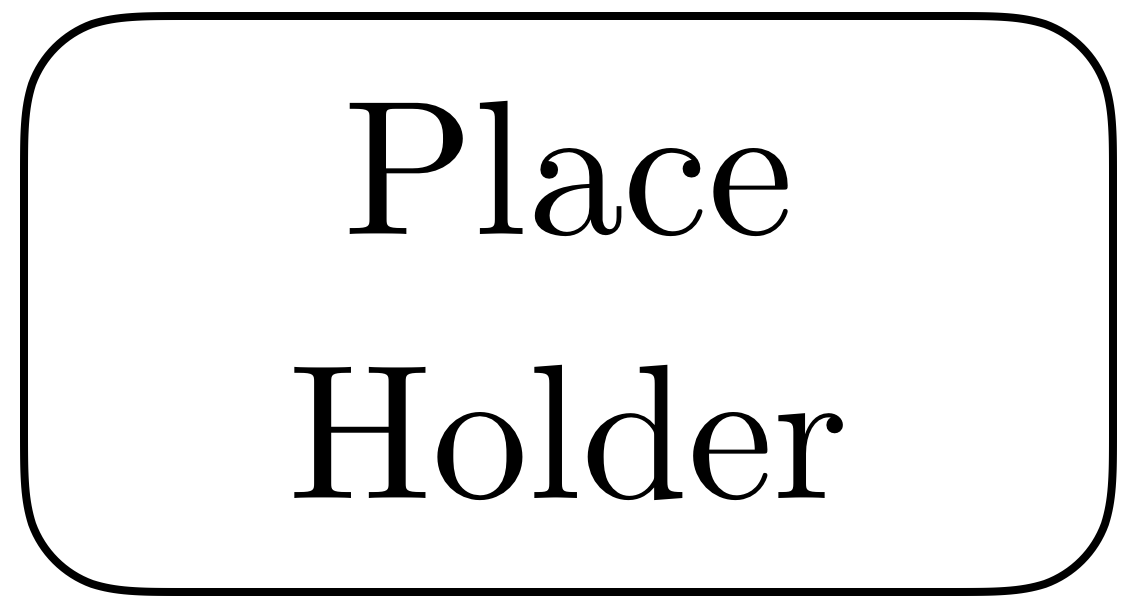
\includegraphics[width=0.28\columnwidth]{figures/placeholder.png}}
\subfigure[NChain]{
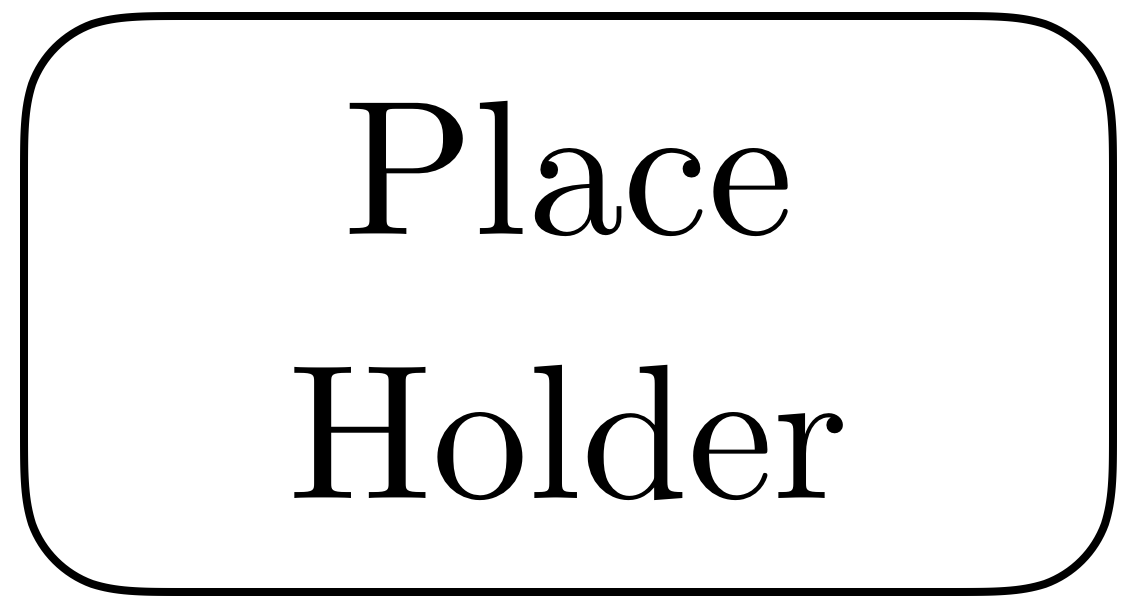
\includegraphics[width=0.28\columnwidth]{figures/placeholder.png}}
\subfigure[Trench]{
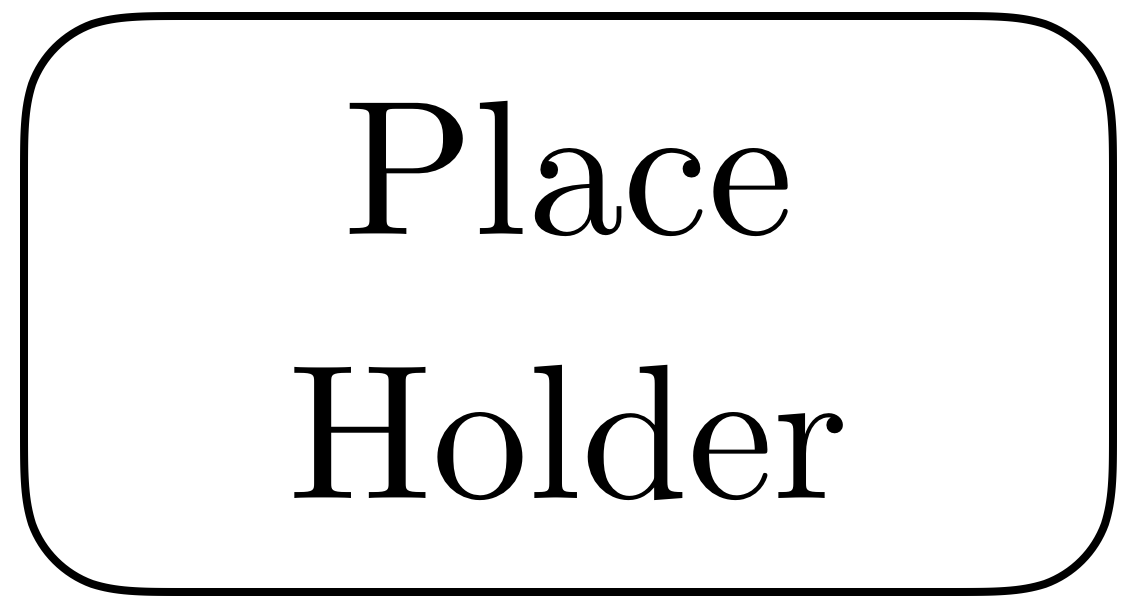
\includegraphics[width=0.28\columnwidth]{figures/placeholder.png}}
\label{fig:eps-states}
\caption{$\epsilon$ vs. Num States}
\end{figure} 

% Figure: Epsilon vs. Error in Abstract Value Function
\begin{figure}
\subfigure[UpWorld]{
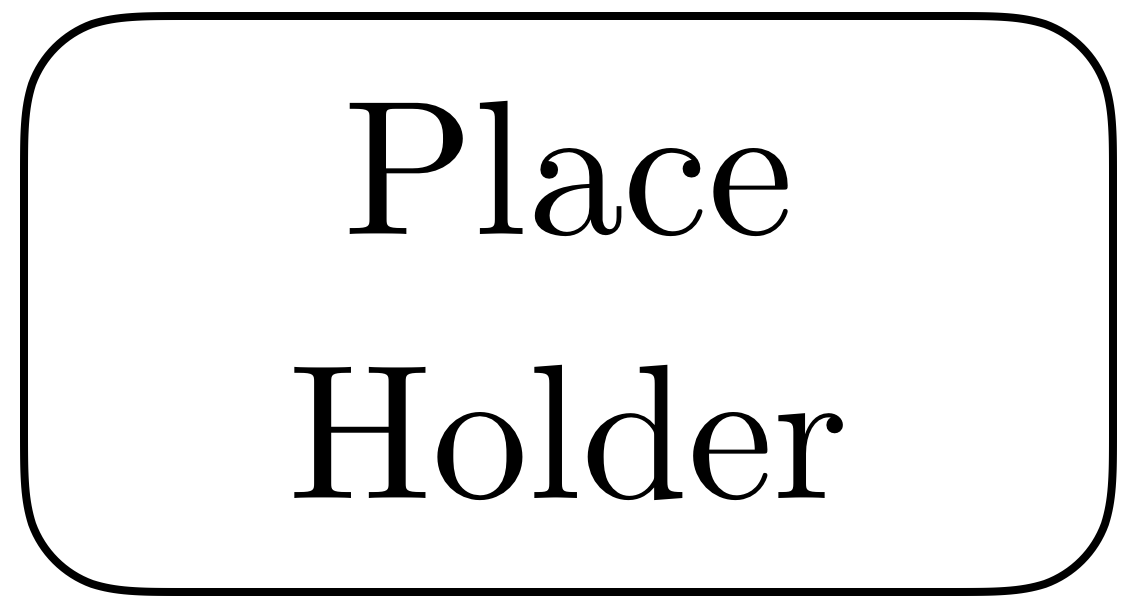
\includegraphics[width=0.28\columnwidth]{figures/placeholder.png}}
\subfigure[NChain]{
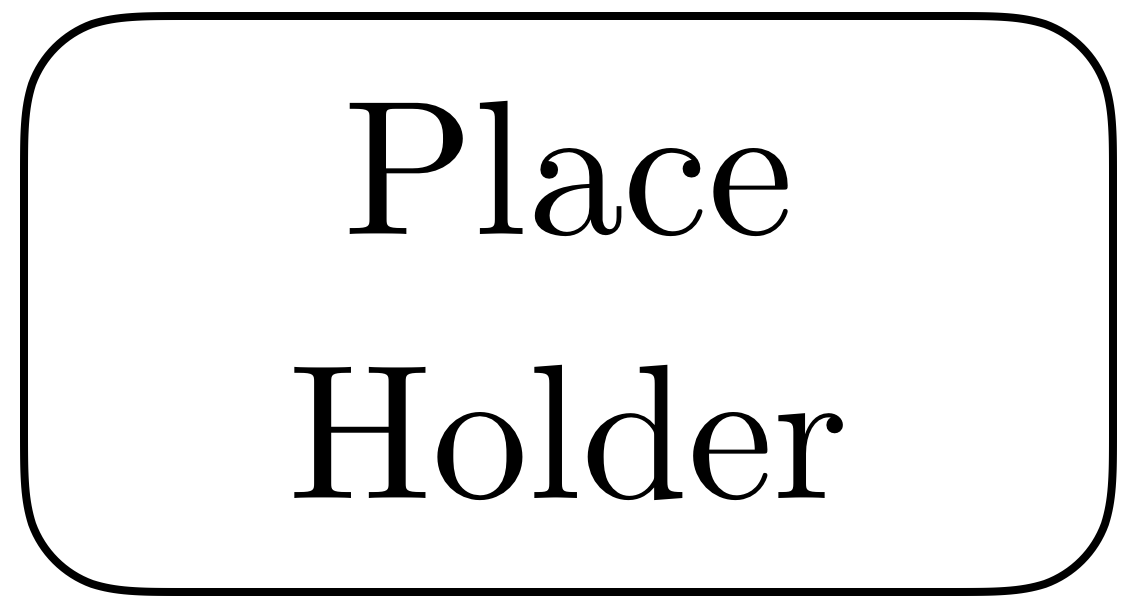
\includegraphics[width=0.28\columnwidth]{figures/placeholder.png}}
\subfigure[Trench]{
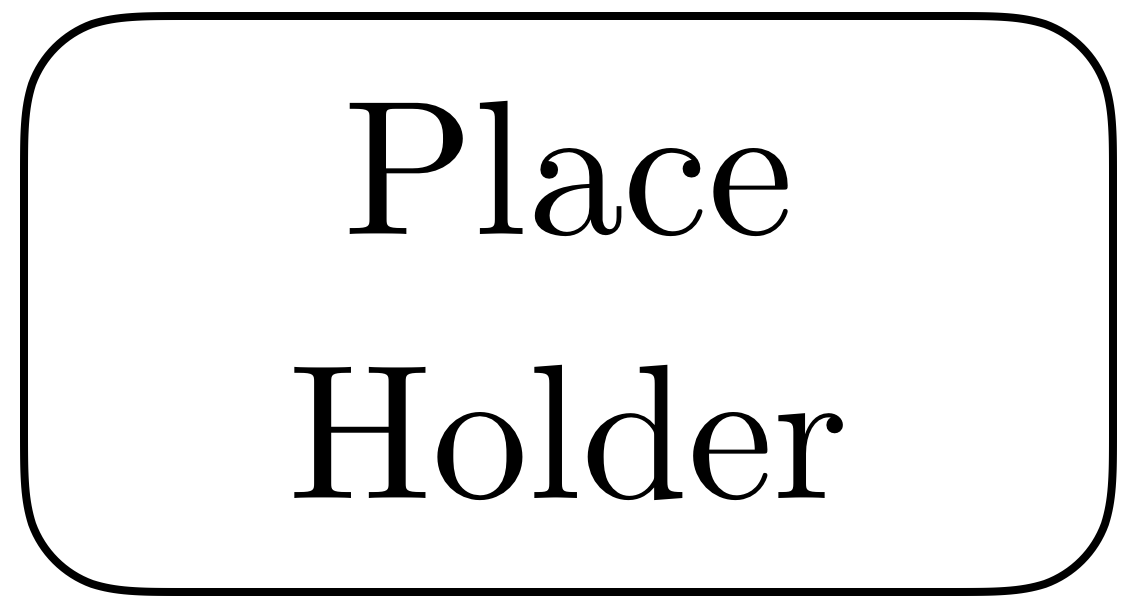
\includegraphics[width=0.28\columnwidth]{figures/placeholder.png}}
\label{fig:eps-states}
\caption{$\epsilon$ vs. Error in Abstract Value Function}
\end{figure} 



% Subsection: Abstract Domain Visualizations
\subsection{Abstract Domain Visualizations}

% Figure: UpWorld MDP visuals
\begin{figure}[h]
\centering
\subfigure[UpWorld]{
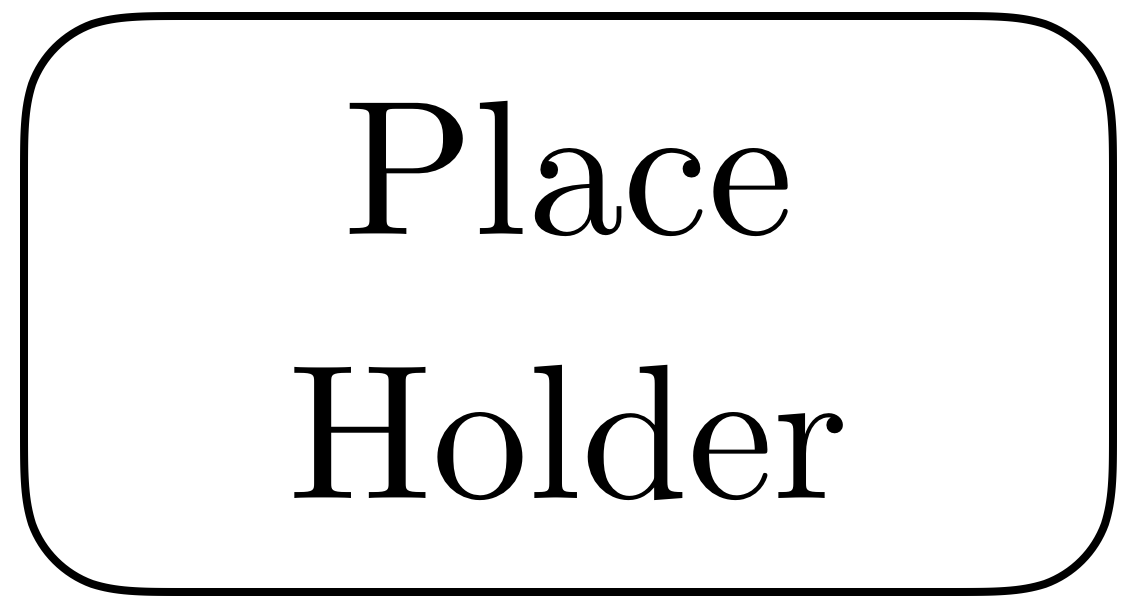
\includegraphics[width=0.46\columnwidth]{figures/placeholder.png}}
\hspace{3mm}
\subfigure[Abstracted UpWorld]{
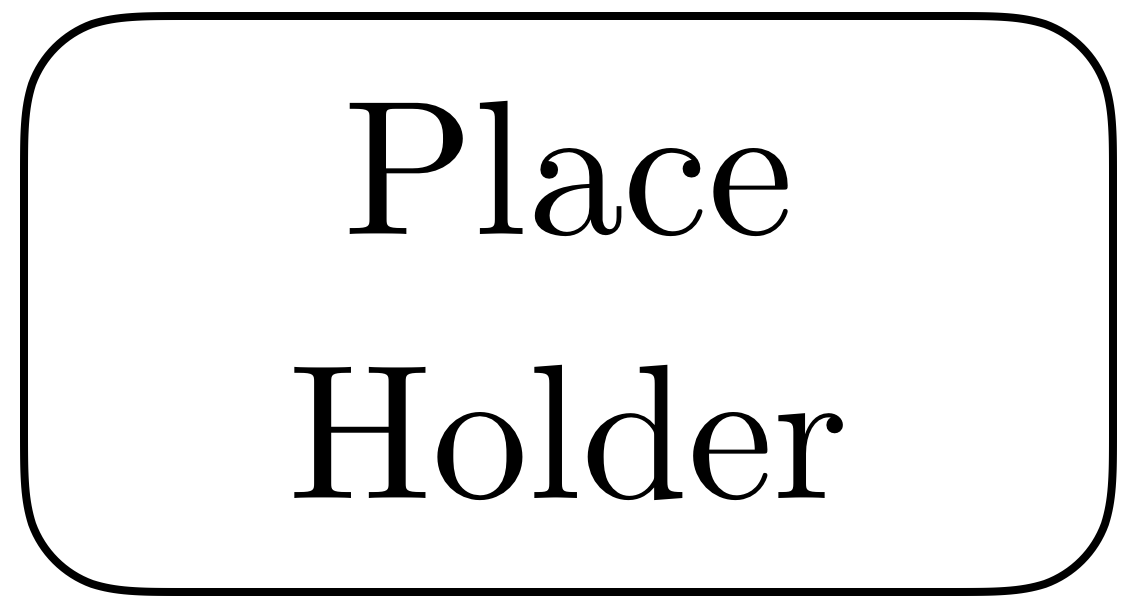
\includegraphics[width=0.46\columnwidth]{figures/placeholder.png}}
\caption{Visualization of Original UpWorld vs. Abstracted UpWorld}
\end{figure}

% Figure: NChain MDP visuals
\begin{figure}[h]
\centering
\subfigure[NChain]{
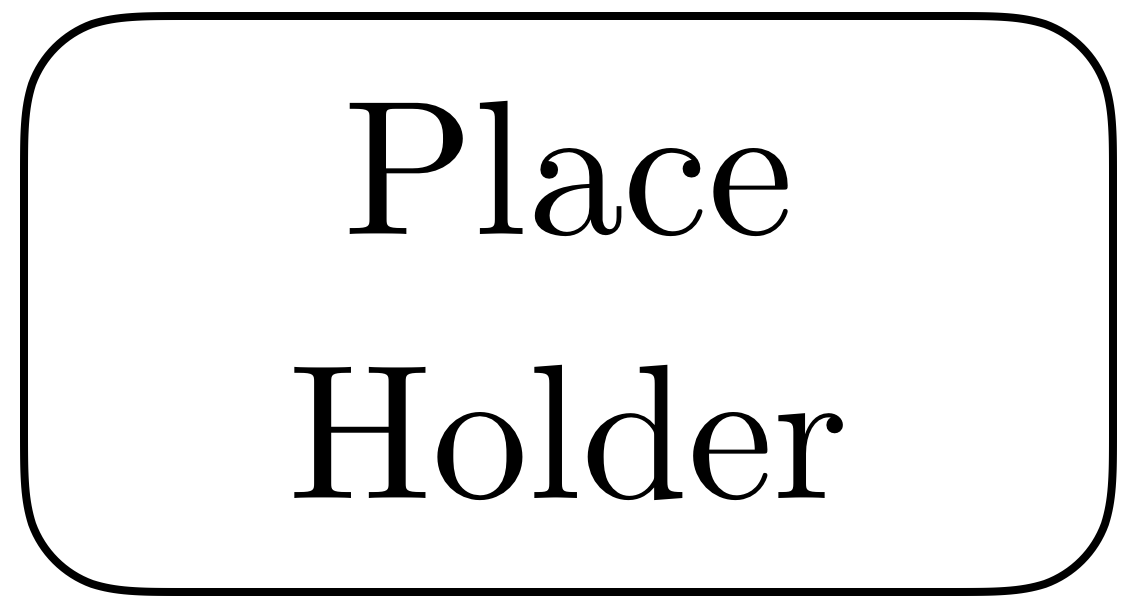
\includegraphics[width=0.46\columnwidth]{figures/placeholder.png}}
\hspace{3mm}
\subfigure[Abstracted NChain ]{
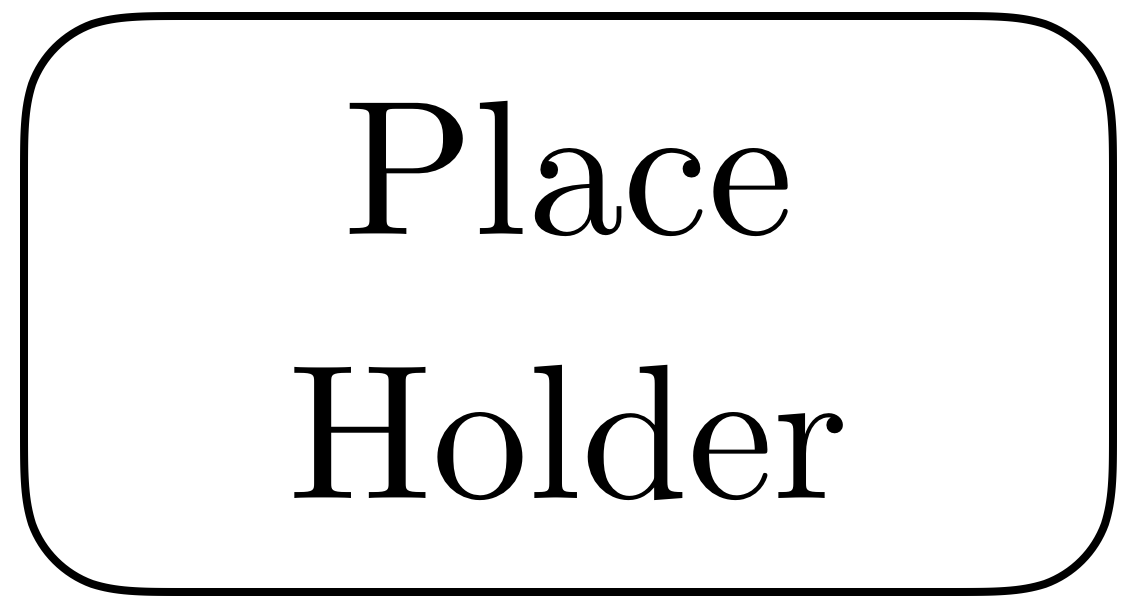
\includegraphics[width=0.46\columnwidth]{figures/placeholder.png}}
\caption{Visualization of Original NChain vs. Abstracted NChain}
\end{figure}






% --- SECTION: Conclusion ---
\section{Conclusion}

% Summary

% Future Work
\begin{enumerate}
\item Learning Phi
\begin{itemize}
\item Exploration vs. Exploitation problem is different while trying to learn Phi
\end{itemize}
\item Compressibility
\begin{itemize}
\item Relationship between approximate abstract and compressibility
\end{itemize}
\item POMDP and abstraction
\end{enumerate}





% --- BIBLIOGRAPHY ---
\bibliographystyle{icml2016/icml2016}
\bibliography{state_abs}

\end{document}
